\documentclass[conference]{IEEEtran}
\IEEEoverridecommandlockouts

\usepackage[utf8]{inputenc}
\usepackage[T1]{fontenc}
\usepackage{cite}
\usepackage{amsmath,amssymb}
\usepackage{booktabs}
\usepackage{tabularx}
\usepackage{array}
\usepackage{graphicx}
\usepackage{url}
\usepackage[hidelinks]{hyperref}
\usepackage{xspace}

\setlength{\textfloatsep}{5pt plus 1.5pt minus 1.5pt}
\setlength{\dbltextfloatsep}{5pt plus 1.5pt minus 1.5pt}
\setlength{\intextsep}{5pt plus 1.5pt minus 1.5pt}
\setlength{\abovecaptionskip}{2.5pt}
\setlength{\belowcaptionskip}{1pt}

% Gerado por paper/gera_tabelas.py. Não editar à mão.
\newcommand{\NumMatrizes}{8\xspace}
\newcommand{\NumExecSpmv}{96\xspace}
\newcommand{\NumBitExatas}{96\xspace}
\newcommand{\MinLinhas}{30\xspace}
\newcommand{\MaxLinhas}{1033\xspace}
\newcommand{\MaxNnz}{6027\xspace}
\newcommand{\MedFPtrinta}{$5.91 \times 10^{-8}$\xspace}
\newcommand{\MedTakumTrinta}{$1.15 \times 10^{-8}$\xspace}
\newcommand{\MedFPtrintaAcSes}{$3.61 \times 10^{-8}$\xspace}
\newcommand{\MedTakumTrintaAcTrinta}{$2.94 \times 10^{-8}$\xspace}
\newcommand{\MedTakumTrintaScaled}{$5.37 \times 10^{-9}$\xspace}
\newcommand{\MedBF}{$2.36 \times 10^{-3}$\xspace}
\newcommand{\MedTakumDez}{$7.43 \times 10^{-4}$\xspace}
\newcommand{\MedTakumDezScaled}{$3.09 \times 10^{-4}$\xspace}
\newcommand{\MedTakumOito}{$1.52 \times 10^{-1}$\xspace}
\newcommand{\MedTakumOitoScaled}{$8.39 \times 10^{-2}$\xspace}
\newcommand{\RazaoFormatoAcTrinta}{2.01\xspace}
\newcommand{\RazaoAcumuladorTakum}{2.56\xspace}
\newcommand{\RazaoKernelTrinta}{5.15\xspace}
\newcommand{\RazaoAcAmpliadoTrinta}{3.15\xspace}
\newcommand{\RazaoTakumBF}{3.17\xspace}
\newcommand{\RazaoTakumBFScaled}{7.61\xspace}
\newcommand{\ParTrintaFPAmbos}{8\xspace}
\newcommand{\ParTrintaFPTakumVence}{7\xspace}
\newcommand{\ParTrintaFPOutroVence}{1\xspace}
\newcommand{\ParTrintaFPEmpates}{0\xspace}
\newcommand{\ParTrintaFPTakumNF}{0\xspace}
\newcommand{\ParTrintaFPOutroNF}{0\xspace}
\newcommand{\ParTrintaAcFPAmbos}{8\xspace}
\newcommand{\ParTrintaAcFPTakumVence}{7\xspace}
\newcommand{\ParTrintaAcFPOutroVence}{1\xspace}
\newcommand{\ParTrintaAcFPEmpates}{0\xspace}
\newcommand{\ParTrintaAcFPTakumNF}{0\xspace}
\newcommand{\ParTrintaAcFPOutroNF}{0\xspace}
\newcommand{\ParDezFPAmbos}{5\xspace}
\newcommand{\ParDezFPTakumVence}{3\xspace}
\newcommand{\ParDezFPOutroVence}{2\xspace}
\newcommand{\ParDezFPEmpates}{0\xspace}
\newcommand{\ParDezFPTakumNF}{0\xspace}
\newcommand{\ParDezFPOutroNF}{3\xspace}
\newcommand{\ParDezBFAmbos}{8\xspace}
\newcommand{\ParDezBFTakumVence}{7\xspace}
\newcommand{\ParDezBFOutroVence}{1\xspace}
\newcommand{\ParDezBFEmpates}{0\xspace}
\newcommand{\ParDezBFTakumNF}{0\xspace}
\newcommand{\ParDezBFOutroNF}{0\xspace}
\newcommand{\ParOitoEquatromAmbos}{4\xspace}
\newcommand{\ParOitoEquatromTakumVence}{0\xspace}
\newcommand{\ParOitoEquatromOutroVence}{4\xspace}
\newcommand{\ParOitoEquatromEmpates}{0\xspace}
\newcommand{\ParOitoEquatromTakumNF}{0\xspace}
\newcommand{\ParOitoEquatromOutroNF}{4\xspace}
\newcommand{\ParOitoCincodoisAmbos}{5\xspace}
\newcommand{\ParOitoCincodoisTakumVence}{3\xspace}
\newcommand{\ParOitoCincodoisOutroVence}{2\xspace}
\newcommand{\ParOitoCincodoisEmpates}{0\xspace}
\newcommand{\ParOitoCincodoisTakumNF}{0\xspace}
\newcommand{\ParOitoCincodoisOutroNF}{3\xspace}
\newcommand{\NFTakumOito}{0\xspace}
\newcommand{\NFTakumDez}{0\xspace}
\newcommand{\NFEquatrom}{4\xspace}
\newcommand{\NFCincodois}{3\xspace}
\newcommand{\NFDez}{3\xspace}
\newcommand{\NFBF}{0\xspace}
\newcommand{\ElemNnzFP}{5.33\xspace}
\newcommand{\ElemNnzTakum}{4.50\xspace}
\newcommand{\InsnNnzFPCento}{6.14\xspace}
\newcommand{\CsrNnzFPCento}{1.33\xspace}
\newcommand{\InsnNnzFPDuzentos}{4.59\xspace}
\newcommand{\CsrNnzFPDuzentos}{1.07\xspace}
\newcommand{\InsnNnzFPQuinhentos}{4.34\xspace}
\newcommand{\CsrNnzFPQuinhentos}{1.03\xspace}
\newcommand{\InsnNnzTrintaCento}{5.98\xspace}
\newcommand{\CsrNnzTrintaCento}{1.33\xspace}
\newcommand{\RelInsnTrintaCento}{$-$2.7\%\xspace}
\newcommand{\RelCsrTrintaCento}{+0.0\%\xspace}
\newcommand{\EconomiaCento}{2.7\%\xspace}
\newcommand{\ZvtNnzTrintaCento}{0.50\xspace}
\newcommand{\InsnNnzTrintaDuzentos}{4.55\xspace}
\newcommand{\CsrNnzTrintaDuzentos}{1.07\xspace}
\newcommand{\RelInsnTrintaDuzentos}{$-$0.7\%\xspace}
\newcommand{\RelCsrTrintaDuzentos}{+0.0\%\xspace}
\newcommand{\EconomiaDuzentos}{0.7\%\xspace}
\newcommand{\ZvtNnzTrintaDuzentos}{0.37\xspace}
\newcommand{\InsnNnzTrintaQuinhentos}{4.33\xspace}
\newcommand{\CsrNnzTrintaQuinhentos}{1.03\xspace}
\newcommand{\RelInsnTrintaQuinhentos}{$-$0.3\%\xspace}
\newcommand{\RelCsrTrintaQuinhentos}{+0.0\%\xspace}
\newcommand{\EconomiaQuinhentos}{0.3\%\xspace}
\newcommand{\ZvtNnzTrintaQuinhentos}{0.35\xspace}
\newcommand{\InsnNnzDezCento}{4.95\xspace}
\newcommand{\CsrNnzDezCento}{1.47\xspace}
\newcommand{\RelInsnDezCento}{$-$19.3\%\xspace}
\newcommand{\RelCsrDezCento}{+10.7\%\xspace}
\newcommand{\ZvtNnzDezCento}{0.37\xspace}
\newcommand{\InsnNnzDezDuzentos}{4.69\xspace}
\newcommand{\CsrNnzDezDuzentos}{1.39\xspace}
\newcommand{\RelInsnDezDuzentos}{+2.2\%\xspace}
\newcommand{\RelCsrDezDuzentos}{+29.9\%\xspace}
\newcommand{\ZvtNnzDezDuzentos}{0.35\xspace}
\newcommand{\InsnNnzDezQuinhentos}{4.60\xspace}
\newcommand{\CsrNnzDezQuinhentos}{1.36\xspace}
\newcommand{\RelInsnDezQuinhentos}{+6.0\%\xspace}
\newcommand{\RelCsrDezQuinhentos}{+32.5\%\xspace}
\newcommand{\ZvtNnzDezQuinhentos}{0.34\xspace}
\newcommand{\InsnNnzOitoCento}{4.51\xspace}
\newcommand{\CsrNnzOitoCento}{1.39\xspace}
\newcommand{\RelInsnOitoCento}{$-$26.6\%\xspace}
\newcommand{\RelCsrOitoCento}{+4.6\%\xspace}
\newcommand{\ZvtNnzOitoCento}{0.35\xspace}
\newcommand{\InsnNnzOitoDuzentos}{4.43\xspace}
\newcommand{\CsrNnzOitoDuzentos}{1.36\xspace}
\newcommand{\RelInsnOitoDuzentos}{$-$3.4\%\xspace}
\newcommand{\RelCsrOitoDuzentos}{+27.4\%\xspace}
\newcommand{\ZvtNnzOitoDuzentos}{0.34\xspace}
\newcommand{\InsnNnzOitoQuinhentos}{4.39\xspace}
\newcommand{\CsrNnzOitoQuinhentos}{1.35\xspace}
\newcommand{\RelInsnOitoQuinhentos}{+1.1\%\xspace}
\newcommand{\RelCsrOitoQuinhentos}{+31.2\%\xspace}
\newcommand{\ZvtNnzOitoQuinhentos}{0.34\xspace}
\newcommand{\InsnMenorTrinta}{13\xspace}
\newcommand{\InsnIgualTrinta}{11\xspace}
\newcommand{\InsnMaiorTrinta}{0\xspace}
\newcommand{\InsnMenorDez}{11\xspace}
\newcommand{\InsnIgualDez}{0\xspace}
\newcommand{\InsnMaiorDez}{13\xspace}
\newcommand{\InsnMenorOito}{12\xspace}
\newcommand{\InsnIgualOito}{0\xspace}
\newcommand{\InsnMaiorOito}{12\xspace}
\newcommand{\InsnPares}{24\xspace}
\newcommand{\ModRFP}{13\xspace}
\newcommand{\ModCFP}{12\xspace}
\newcommand{\ModKFP}{21\xspace}
\newcommand{\ModROito}{14\xspace}
\newcommand{\ModCOito}{12\xspace}
\newcommand{\ModKOito}{21\xspace}
\newcommand{\ModRDez}{14\xspace}
\newcommand{\ModCDez}{13\xspace}
\newcommand{\ModKDez}{21\xspace}
\newcommand{\ModRTrinta}{14\xspace}
\newcommand{\ModCTrinta}{11\xspace}
\newcommand{\ModKTrinta}{21\xspace}
\newcommand{\ModExatas}{96\xspace}
\newcommand{\ModExec}{96\xspace}
\newcommand{\ModSinteticosOk}{12\xspace}
\newcommand{\ModSinteticosTotal}{12\xspace}
\newcommand{\ModResiduoMax}{0\xspace}


\author{\IEEEauthorblockN{Andr\'e Lu\'is Alves Rezende, Gabriel Ramos Fontes,
Isadora Maria Carvalho Lopes, Jo\~ao Pedro Santos de Brito}
\IEEEauthorblockA{Department of Electronic Engineering (DELT), Federal University of Minas Gerais (UFMG)\\
Belo Horizonte, MG, Brazil}}

\title{Implementation and Evaluation of Takum Arithmetic in the RISC-V Vector Extension (Zvtakum)}

\begin{document}
\maketitle

\begin{abstract}
Low-precision floating-point formats (IEEE FP16, bfloat16, OCP FP8 E4M3/E5M2) expand vector instruction sets with fragmented decoders, subnormal datapaths, cross-format conversions, and floating-point control/status hazards. Takum arithmetic combines tapered precision, a bounded dynamic range, and a fixed 12-bit most-significant decoding window across element widths. We present \texttt{Zvtakum}, an experimental RISC-V Vector (RVV~1.0) extension supporting \texttt{T8}, \texttt{T16}, and \texttt{T32} via five \texttt{custom-0} instructions: \texttt{vtadd.vv}, \texttt{vtsub.vv}, \texttt{vtmul.vv}, \texttt{vtdot.vv} (double-width accumulation), and \texttt{vncvt.t.t} (narrowing). We implement a 128-bit integer Takum ALU with code-space round-to-nearest-even (RNE) rounding inside a functional RV64IM, Zicsr, RVV~1.0, and \texttt{Zvtakum} simulator. Verification covers 81 C++ checks (52 core, 29 simulator), 75 Python unit tests, exhaustive \texttt{T8} tables and 80,000 \texttt{T16/T32} checks against \texttt{libtakum}, 6,017 \texttt{binary128} oracle checks against \texttt{libquadmath}, differential runs against QEMU~10.2.2 across $\mathrm{VLEN}\in\{128,256,512\}$, and \NumExecSpmv\ bitwise-exact Sparse Matrix-Vector (SpMV) runs on eight Harwell-Boeing matrices. With equal 32-bit accumulators, \texttt{Takum32} lowers median relative $\ell_2$ SpMV error by $\RazaoFormatoAcTrinta\times$ over \texttt{FP32} (and $\RazaoKernelTrinta\times$ with \texttt{T64} accumulation). Unlike unscaled \texttt{E4M3}, \texttt{E5M2}, and \texttt{FP16}, which suffer non-finite overflows on 3 or 4 of 8 matrices, \texttt{Takum8} and \texttt{Takum16} remain 100\% finite while \texttt{Takum16} lowers error relative to \texttt{bfloat16} in 7/8 unscaled and 8/8 scaled runs; by contrast, \texttt{Posit8,2} outperforms \texttt{Takum8} on 7/8 matrices near unity. An analytic model ($N_f = r_f R + c_f S + K$) matches all simulated runs with zero residual, showing that \texttt{Takum32} never exceeds \texttt{FP32} instruction counts.
\end{abstract}

\begin{IEEEkeywords}
RISC-V, RVV, Takum arithmetic, tapered precision, Zvtakum, SpMV, functional simulator.
\end{IEEEkeywords}

\section{Introduction}
Vector and Single Instruction, Multiple Data (SIMD) processors for machine learning and sparse linear algebra are often constrained by memory bandwidth. Packing more operands into fixed vector registers has motivated multiple low-precision IEEE~754 derivatives, including half-precision (\texttt{FP16}), brain floating point (\texttt{bfloat16})~\cite{bfloat16}, and Open Compute Project 8-bit formats (\texttt{OFP8 E4M3} and \texttt{E5M2})~\cite{ofp8,micikevicius2022fp8}. However, fixed-split binary layouts force a rigid trade-off between dynamic range and significand width, introducing incompatible sub-formats, subnormal alignment paths, multiple NaN encodings, and $O(N^2)$ cross-conversion instructions~\cite{hunhold2025avx102}. In the RISC-V Vector Extension (RVV~1.0)~\cite{riscv-v-spec}, \texttt{FP8} is not standardized, \texttt{FP16} requires \texttt{Zvfh}, and \texttt{bfloat16} adds dedicated conversion extensions (\texttt{Zvfbfmin} and \texttt{Zvfbfwma}).

Takum arithmetic~\cite{hunhold2024takum} addresses these issues through tapered precision and a bounded 12-MSB non-fractional prefix across all bit widths. Building on Hunhold's AVX10.2 streamlining study~\cite{hunhold2025avx102}, this work specifies, implements, and evaluates \texttt{Zvtakum} over RVV~1.0 with four contributions:
\begin{enumerate}
    \item A 128-bit integer Takum codec and ALU for \texttt{T8}, \texttt{T16}, and \texttt{T32} (\texttt{T64} accumulation) implementing Definition~8 linear semantics and code-space RNE without host floating-point intermediates;
    \item The \texttt{Zvtakum} ISA using five \texttt{custom-0} instructions integrated into a RISC-V/RVV datapath without \texttt{fcsr} rounding or exception dependencies;
    \item Multi-layer verification spanning exact rationals, \texttt{libtakum}, \texttt{libquadmath}, and differential execution against QEMU~10.2.2~\cite{qemu};
    \item SpMV ($y = A\cdot x$) and 100-matrix SuiteSparse evaluations comparing \texttt{Takum} against \texttt{FP32}, \texttt{FP16}, \texttt{bfloat16}, \texttt{OFP8} (standard and saturating), \texttt{pow2-bound} scaling, \texttt{Posit} (\texttt{es=2}), and logarithmic Takum.
\end{enumerate}

\section{Theoretical Background}

\subsection{Low-Precision IEEE Derivatives and Posit Arithmetic}
IEEE~754 binary formats~\cite{ieee754} partition words into fixed sign, exponent, and fraction fields. \texttt{FP16} (10 fraction bits) provides fine local resolution near unity, yet its dynamic range ($\approx 10^{\pm 5}$) overflows without external scaling. The \texttt{bfloat16} format~\cite{bfloat16} retains the 8-bit exponent of \texttt{FP32} ($\approx 10^{\pm 38}$) with 7 fraction bits, whereas \texttt{OFP8} splits 8-bit workloads into \texttt{E4M3} ($[-448,448]$) and \texttt{E5M2} ($[-57344,57344]$)~\cite{ofp8}. Posit arithmetic~\cite{gustafson2017posit} offers tapered precision with two special patterns ($0$ and \texttt{NaR}), yet its unary regime requires full-word leading-zero/one detectors and \texttt{Posit8} ($es=2$) is bounded to $[2^{-24}, 2^{24}]$ ($\approx 10^{\pm 7.2}$).

\begin{figure*}[t]
\centering
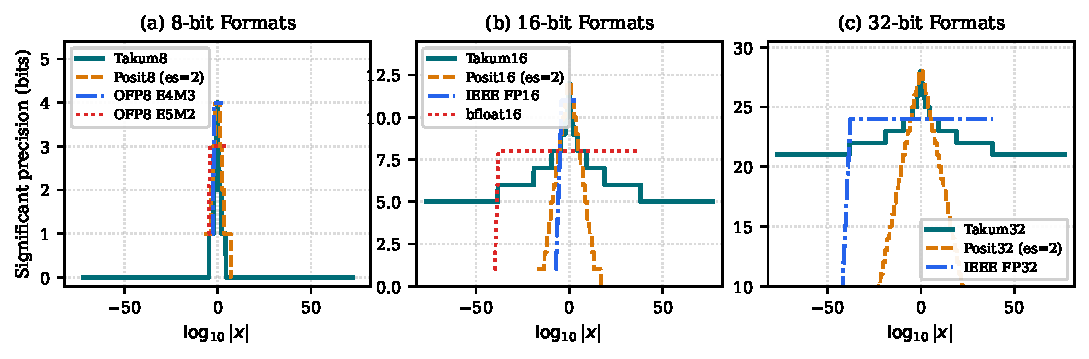
\includegraphics[width=0.72\textwidth]{figures/tapered-precision.pdf}
\caption{Significant precision ($1+p$ bits) vs.\ scale ($\log_{10}|x|$, \texttt{symlog} on $|\log_{10}|x||\le 5$) across 8--32 bits. Centrally, \texttt{Posit} ($es=2$) keeps higher moderate-range precision and \texttt{OFP8}/\texttt{FP16} end by $\pm 4.8$, while Takum spans $\approx 10^{\pm 72}$--$10^{\pm 77}$ via 12~MSBs.}
\label{fig:tapered}
\end{figure*}

\subsection{Takum Encoding and Unified 12-MSB Window}
An $n$-bit Takum word $X[n-1:0]$ packs sign $S$ (1 bit), direction $D$ (1 bit), regime $R$ (3 bits), variable characteristic $C$ ($r$ bits), and fraction $F$ ($p = n - 5 - r$ bits) from MSB to LSB~\cite{hunhold2024takum}. Reserved values are $0\dots0$ (zero) and $10\dots0$ (\texttt{NaR}), with no signed zero or infinity; two's-complement negation preserves total order. Regime width $r \in \{0,\dots,7\}$ depends only on $D$ and $R$:
\begin{equation}
    r = \begin{cases} 7 - \mathrm{uint}(R), & D = 0 \\ \mathrm{uint}(R), & D = 1 \end{cases},\quad
    L_{\max} = 5 + 7 = 12~\text{bits}.
\end{equation}
Since $r \le 7$, the scale prefix $(S, D, R, C)$ fits within the 12 MSBs at every bit width. For $n < 12$ (\texttt{T8}), left-shifting by $12 - n = 4$ bits appends phantom zero (ghost) bits on the right~\cite{hunhold2024takum}, bounding the \texttt{T8} exponent to $[-239, +239]$ ($\approx 10^{\pm 72}$) while sharing identical decoder logic across \texttt{T8}, \texttt{T16}, and \texttt{T32}.

In the linear Takum variant (Definition~8 of~\cite{hunhold2024takum}) selected for our vector ALU, signed characteristic $c$ and value $v$ are:
\begin{equation}
    c = \begin{cases} -(2^{r+1}-1) + \mathrm{uint}(C), & D = 0 \\ (2^r - 1) + \mathrm{uint}(C), & D = 1 \end{cases},
\end{equation}
\begin{equation}
    v = (-1)^S \left(1 - 3S + \frac{\mathrm{uint}(F)}{2^p}\right) \cdot 2^{(-1)^S (c + S)},
\end{equation}
which decomposes into integer significand $N = 2^p + F$ ($S=0$) or $N = 2^{p+1} - F$ ($S=1$) scaled by $2^{c-p}$ or $2^{-(c+1)-p}$. Using a \texttt{symlog} axis centered on $|\log_{10}|x||\le 5$, Figure~\ref{fig:tapered} exposes the central-region trade-off: at $|x|\in[0.5,2)$, \texttt{Takum} and \texttt{Posit} ($es=2$) tie at $n-4$ significant bits (4, 12, and 28, above \texttt{FP16}, \texttt{bfloat16}, and \texttt{FP32}). Across $0.3\lesssim|\log_{10}|x||\lesssim 4.8$, Takum's fixed $(D,R)$ bits expand $r$ right past $2^{\pm 1}$, whereas \texttt{Posit}'s compact unary prefix keeps 1 to 2 extra bits over $[2^{-4},2^4)$ before dropping sharply; past $|\log_{10}|x||\le 5$, \texttt{OFP8}/\texttt{FP16} overflow while \texttt{Takum16/32} sustain 5- and 21-bit floors out to $\approx 10^{\pm 77}$. Conversely, logarithmic Takum (Definition~2~\cite{hunhold2024takum}, $v = (-1)^S \exp(\ell/2)$) turns multiplies/inversions into integer additions (41.2\% in \texttt{T8} and 36.7\% in \texttt{T16} multiplicative closure vs.\ 33.7\% and 1.2\% for linear Takum), yet needs $\Delta_\pm$ lookup tables for addition, whereas linear Takum matches RVV integer lanes~\cite{hunhold2025avx102}.

\section{Related Work}
Hunhold~\cite{hunhold2025avx102} showed that replacing multiple SIMD formats in Intel AVX10.2 with Takum simplifies opcode tables and improves accuracy across 1,401 SuiteSparse matrices~\cite{davis2011suitesparse,mufolab}. His VHDL Takum codec~\cite{hunhold2024vhdl} achieved up to 38\% lower latency and 50\% fewer LUTs than posit codecs. Follow-up studies on sparse linear solvers~\cite{hunhold2025solvers}, implicitly restarted Arnoldi eigensolvers~\cite{hunhold2025arnoldi}, and consecutive integer representations~\cite{hunhold2025integers} evaluated Takum against \texttt{bfloat16}, \texttt{OFP8}, and posits in software. Within RISC-V, PERCIVAL~\cite{mallasen2022percival} and Cococcioni et al.~\cite{cococcioni2021vectorizing} integrated scalar and vector posit units with quires; FPnew~\cite{mach2020fpnew} and FAUST~\cite{kovac2023faust} built transprecision IEEE vector FPUs; and Marcelli et al.~\cite{marcelli2025fp8spike} extended the Spike simulator with 8-bit SoftFloat instructions. Our \texttt{Zvtakum} design differs by targeting unified-width Takum vector arithmetic over RVV~1.0 using an exact 128-bit integer ALU and differential validation against QEMU and \texttt{libtakum}.

\section{Methodology and Proposed Architecture}

\subsection{RVV Restructuring and \texttt{Zvtakum} Encoding}
An audit of \texttt{riscv-opcodes}~\cite{riscv-opcodes} counts 510 vector instructions across RVV~1.0, \texttt{bfloat16} (\texttt{Zvfbfmin}/\texttt{Zvfbfwma}), and vector crypto (\texttt{Zvk*}), including 92 FP and 4 \texttt{bfloat16} ops (25 conversions). Following the AVX10.2 consolidation methodology~\cite{hunhold2025avx102}, parameterizing \texttt{T8}/\texttt{T16}/\texttt{T32} via \texttt{vtype.vsew} collapses those 96 FP/conversion operations into eight core Takum primitives (\texttt{vtadd}, \texttt{vtsub}, \texttt{vtmul}, \texttt{vtdiv}, \texttt{vtsqrt}, \texttt{vtdot}, \texttt{vncvt.t.t}, and integer conversions), while comparisons reuse standard two's-complement integer vector ops~\cite{hunhold2024takum}.

\begin{table}[t]
\caption{Proposed \texttt{Zvtakum} Instructions in \texttt{custom-0} (\texttt{0x0B}, \texttt{funct3=000}).}
\label{tab:zvtakum_isa}
\centering
\scriptsize
\begin{tabular}{@{}llll@{}}
\toprule
Mnemonic & funct6 & RVV Equiv. & Operational Semantics \\
\midrule
\texttt{vtadd.vv} & \texttt{000000} & \texttt{vfadd.vv} & $vd[i] = vs2[i] + vs1[i]$ (\texttt{SEW}) \\
\texttt{vtsub.vv} & \texttt{000001} & \texttt{vfsub.vv} & $vd[i] = vs2[i] - vs1[i]$ (\texttt{SEW}) \\
\texttt{vtmul.vv} & \texttt{000010} & \texttt{vfmul.vv} & $vd[i] = vs2[i] \times vs1[i]$ (\texttt{SEW}) \\
\texttt{vtdot.vv} & \texttt{000011} & \texttt{vfdot.vv} & $vd[0]_{2\mathrm{SEW}} \mathrel{+}= \sum_i vs2[i]\cdot vs1[i]$ \\
\texttt{vncvt.t.t} & \texttt{000100} & \texttt{vfncvt.*} & $vd[i]_{\mathrm{SEW}} = \mathrm{narrow}(vs2[i]_{2\mathrm{SEW}})$ \\
\bottomrule
\end{tabular}
\vspace{2pt}
\raggedright\footnotesize{Encodings in \texttt{custom-0} (\texttt{funct6}=0..4); bit~25 (\texttt{vm}) selects mask \texttt{v0}; \texttt{vncvt.t.t} requires \texttt{vs1=00000}.}
\end{table}

Table~\ref{tab:zvtakum_isa} lists the five implemented instructions. Earlier drafts considered overloading a single \texttt{OP-V} slot (\texttt{funct6=0b111001}), assuming it was uniquely free; checking \texttt{riscv-opcodes} showed 11 to 33 unallocated \texttt{funct6} slots reserved for standard extensions. We therefore allocate \texttt{Zvtakum} in RISC-V's \texttt{custom-0} space (\texttt{opcode=0x0B}, \texttt{funct3=000}, \texttt{funct6=0..4}), leaving \texttt{OP-V} untouched. Element-wise ops support $\mathrm{SEW}\in\{8,16,32\}$ and $\mathrm{LMUL}\in\{1,2,4,8\}$, obeying \texttt{vl}, \texttt{vstart}, mask \texttt{v0.t}, and RVV~1.0 tail/mask agnostic policies (\texttt{vta}/\texttt{vma}). Instruction \texttt{vtdot.vv} accumulates active products sequentially into \texttt{vd[0]} at $\mathrm{EEW}=2\cdot\mathrm{SEW}$ ($\mathrm{EMUL}=1$), enabling internal \texttt{T64} accumulation for \texttt{T32} without exposing 64-bit vector registers; two roundings occur per step (wide product, then sum). Instruction \texttt{vncvt.t.t} narrows an aligned $2\cdot\mathrm{LMUL}$ source group back to \texttt{SEW}.

\subsection{RISC-V + \texttt{Zvtakum} Datapath and 128-Bit Integer ALU}
\begin{figure*}[t]
\centering
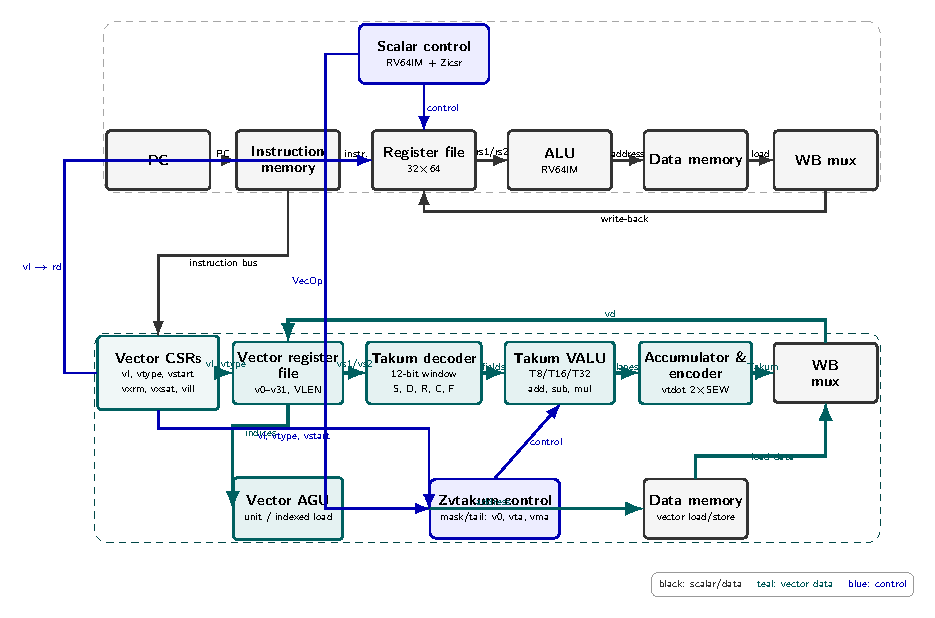
\includegraphics[width=0.90\textwidth]{figures/zvtakum-datapath.pdf}
\caption{Proposed RISC-V datapath extended with the \texttt{Zvtakum} vector subsystem (teal). Scalar core registers supply \texttt{vl}/\texttt{vtype} via \texttt{rs1}, while vector operands pass through a shared 12-MSB Takum decoder, SIMD VALU lanes, a $2\cdot\text{SEW}$ accumulator/narrowing encoder, and vector write-back (\texttt{MuxVWB}). Detailed stage schematics reside in \texttt{figures/datapath\_zvtakum.pdf}.}
\label{fig:datapath}
\end{figure*}

Figure~\ref{fig:datapath} depicts the RISC-V + \texttt{Zvtakum} datapath: \texttt{vsetvl*} updates \texttt{vl}, \texttt{vtype}, and \texttt{vstart}; \texttt{VReg} holds 32 $\mathrm{VLEN}$-bit registers; the unified 12-MSB decoder extracts $[S,D,R,C,F]$ uniformly across \texttt{T8}/\texttt{T16}/\texttt{T32}; and fixed RNE saturation with algebraic \texttt{NaR} eliminates \texttt{fcsr} (\texttt{frm}/\texttt{fflags}) hazards.

Our C++17 Takum ALU (\texttt{src/takum.cpp}) operates strictly in \texttt{uint64\_t} and \texttt{unsigned \_\_int128}, avoiding host \texttt{double} rounding. Decoding yields $(\mathrm{neg}, e, \mathrm{sig})$ representing $(-1)^{\mathrm{neg}}\cdot\mathrm{sig}\cdot 2^{e-63}$. Addition aligns operands across 128 bits with sticky tracking (reused as borrow in effective subtraction); multiplication computes an exact 128-bit product and sticky bit. Positive encoding packs $(D,R,C)$ and $\mathrm{sig}$ into \texttt{u128}, extracts prefix $L$ ($n$ bits), midpoint bit $m$, and sticky $\mathit{st}$, rounds $L \to L+1$ iff $m=1 \land (\mathit{st} \lor (L\bmod 2 = 1))$, clamps to $[1, 2^{n-1}-1]$, and applies two's complement when $\mathrm{neg}=1$, matching Hunhold's hardware spec~\cite{hunhold2024vhdl}.

\section{Verification and Experimental Methodology}

\subsection{Multi-Layer Verification}
Four verification layers validate bitwise equivalence:
\begin{enumerate}
    \item Codec and ALU vs.\ Exact Rationals: Exhaustive \texttt{T8} (\texttt{add}, \texttt{sub}, \texttt{mul}; $3\times 65{,}536$ pairs), \texttt{T16$\to$T8} ($65{,}536$ narrowings), \texttt{T8}/\texttt{T16} round-trips, sampled 200,000 \texttt{T32} round-trips, \texttt{T32$\to$T16/T8} narrowings, algebraic identities, illegal \texttt{custom-0} trapping, and RVV~1.0~\S3.11 \texttt{vtype.vill=1} reset behavior across 81 C++ checks (52 core in \texttt{takum-test}, 29 simulator in \texttt{zt-test}) and 75 Python unit tests (0 failures).
    \item \texttt{libtakum} and Double-Rounding: All 256 \texttt{T8} decodes, 196,608 \texttt{T8} ops, 65,536 \texttt{T16} decodes, and 50,000 \texttt{T16} ops match \texttt{libtakum}~v2.0.0~\cite{libtakum} (0 mismatches). Across 30,000 \texttt{T32} ops (10,000 per op), \texttt{add} and \texttt{sub} show 0 mismatches while 128 out of 10,000 \texttt{T32} multiplications (all on deliberate tie-probe pairs such as $\texttt{0x40000001} \times \texttt{0x44000001}$) differ by 1~ULP because \texttt{libtakum} passes products through host \texttt{binary64} before encoding.
    \item \texttt{binary128} Oracle: Python exact-rational \texttt{BINARY128} matches GCC~9.4.0 \texttt{\_\_float128}/\texttt{libquadmath} across 6,017 checks (2,000 random/corner pairs $\times$ 3 ops + 17 decimal conversions; 3 documented signed-zero normalizations).
    \item Simulator vs.\ QEMU~10.2.2: \texttt{zt-sim} matches \texttt{qemu-riscv64}~10.2.2 byte-for-byte across 9 runs ($\mathrm{VLEN}\in\{128,256,512\}$) on \texttt{rvv\_std}, \texttt{scalar\_ops}, and \texttt{zvtakum\_isa}. Because RVV~1.0~\S3.11 sets \texttt{vtype.vill=1} on hardware reset (matched by \texttt{zt-sim} and QEMU~10.2.2, verified directly in \texttt{zt-test}) whereas QEMU~8.2.2 user-mode leaves pre-\texttt{vsetvli} \texttt{vtype=0}, \texttt{scalar\_ops} avoids reading uninitialized \texttt{vtype} while \texttt{rvv\_std} verifies configured \texttt{vtype}/\texttt{vl} after \texttt{vsetvli}.
\end{enumerate}

\subsection{SpMV Kernel Design, Scaling, and SuiteSparse Benchmarks}
We evaluate CSR SpMV ($y = A\cdot x$) across eight Harwell-Boeing matrices~\cite{duff1989hb} (\texttt{bcsstk01}, \texttt{bcsstk02}, \texttt{jpwh\_991}, \texttt{pores\_1}, \texttt{sherman1}, \texttt{well1033}, \texttt{west0067}, \texttt{west0132}; $\MinLinhas$ to $\MaxLinhas$ rows, up to $\MaxNnz$ nonzeros) with deterministic vector $x_j = k_j/2^{52}$ ($\text{seed}=2026$). Both \texttt{FP32} and \texttt{Takum} kernels share identical scalar loops and indexed gathers (\texttt{vluxei32.v}): \texttt{FP32} issues 12 instructions/strip (\texttt{vfmul.vv} + \texttt{vfredusum.vs}), whereas \texttt{Takumn} issues \texttt{vtdot.vv} per strip (switching index \texttt{EMUL} for $n\in\{8,16\}$) plus \texttt{vncvt.t.t} once per row. For \texttt{OFP8} (\texttt{E4M3}, \texttt{E5M2}, plus saturating \texttt{E4M3\_sat}/\texttt{E5M2\_sat}), \texttt{FP16}, \texttt{bfloat16}, and \texttt{Posit} (\texttt{es=2}), we compute exact-rational numeric baselines against IEEE \texttt{binary128} (\texttt{Float128}, 113-bit significand) under both unscaled (\texttt{none}) and \texttt{pow2-bound} input scaling. We also report the 100-matrix SuiteSparse conversion benchmark (declared $\mathrm{nnz}\le 50{,}000$; 15 formats evaluated against 80-bit \texttt{long double} in the C11 run, alongside a Python \texttt{binary128} generator and hash-verified manifest validated locally on the eight Harwell-Boeing matrices).

\section{Results and Discussion}

\begin{table*}[t]
\caption{Relative $\ell_2$ SpMV error at 32 bits (VLEN = 256) against Float128, by matrix. FP32 and Takum32 are simulated RISC-V kernels (32-bit and 64-bit accumulators, respectively); controls isolate accumulator width and \texttt{pow2-bound} input scaling.}
\label{tab:precisao32}
\centering
\footnotesize
\begin{tabular}{@{}lrccccc@{}}
\toprule
Matrix & nnz & FP32 (32b acc.) & Takum32 (64b acc.) & FP32 (64b acc.) & Takum32 (32b acc.) & Takum32 (scaled) \\
\midrule
bcsstk01 & 400 & $7.20 \times 10^{-8}$ & $5.06 \times 10^{-8}$ & $3.57 \times 10^{-8}$ & $6.22 \times 10^{-8}$ & $3.54 \times 10^{-9}$ \\
bcsstk02 & 4356 & $1.81 \times 10^{-7}$ & $1.88 \times 10^{-8}$ & $4.63 \times 10^{-8}$ & $8.32 \times 10^{-8}$ & $7.40 \times 10^{-9}$ \\
jpwh\_991 & 6027 & $6.32 \times 10^{-8}$ & $4.19 \times 10^{-9}$ & $3.47 \times 10^{-8}$ & $9.40 \times 10^{-9}$ & $4.38 \times 10^{-9}$ \\
pores\_1 & 180 & $3.54 \times 10^{-8}$ & $7.87 \times 10^{-8}$ & $3.26 \times 10^{-8}$ & $5.44 \times 10^{-8}$ & $5.11 \times 10^{-9}$ \\
sherman1 & 3750 & $5.82 \times 10^{-8}$ & $4.02 \times 10^{-9}$ & $3.65 \times 10^{-8}$ & $4.93 \times 10^{-9}$ & $5.62 \times 10^{-9}$ \\
well1033 & 4732 & $5.99 \times 10^{-8}$ & $4.07 \times 10^{-9}$ & $3.72 \times 10^{-8}$ & $6.45 \times 10^{-9}$ & $6.94 \times 10^{-9}$ \\
west0067 & 294 & $4.82 \times 10^{-8}$ & $3.59 \times 10^{-9}$ & $3.27 \times 10^{-8}$ & $4.84 \times 10^{-9}$ & $6.18 \times 10^{-9}$ \\
west0132 & 413 & $5.01 \times 10^{-8}$ & $3.21 \times 10^{-8}$ & $4.00 \times 10^{-8}$ & $4.94 \times 10^{-8}$ & $2.72 \times 10^{-9}$ \\
\midrule
Median & & $5.91 \times 10^{-8}$ & $1.15 \times 10^{-8}$ & $3.61 \times 10^{-8}$ & $2.94 \times 10^{-8}$ & $5.37 \times 10^{-9}$ \\
\bottomrule
\end{tabular}
\end{table*}

\begin{table*}[t]
\caption{Relative $\ell_2$ SpMV error at 8 and 16 bits against Float128 (VLEN = 256). NF($k$) denotes $k$ non-finite rows (overflow). Accumulators: 16-bit for E4M3, E5M2, Takum8; 32-bit for FP16, BF16, Takum16. Bottom rows summarize finite counts and \texttt{pow2-bound} scaling.}
\label{tab:precisao816}
\centering
\footnotesize
\begin{tabular}{@{}lcccccc@{}}
\toprule
Matrix & E4M3 & E5M2 & FP16 & bfloat16 & Takum16 & Takum8 \\
\midrule
bcsstk01 & NF(48) & NF(48) & NF(48) & $2.28 \times 10^{-3}$ & $3.24 \times 10^{-3}$ & $6.44 \times 10^{-1}$ \\
bcsstk02 & NF(66) & $7.31 \times 10^{-2}$ & $3.76 \times 10^{-4}$ & $2.43 \times 10^{-3}$ & $1.20 \times 10^{-3}$ & $2.27 \times 10^{-1}$ \\
jpwh\_991 & $3.45 \times 10^{-2}$ & $7.58 \times 10^{-2}$ & $2.77 \times 10^{-4}$ & $2.26 \times 10^{-3}$ & $3.04 \times 10^{-4}$ & $7.77 \times 10^{-2}$ \\
pores\_1 & NF(30) & NF(15) & NF(15) & $1.53 \times 10^{-3}$ & $1.18 \times 10^{-3}$ & $8.58 \times 10^{-1}$ \\
sherman1 & $3.95 \times 10^{-2}$ & $1.00 \times 10^{-1}$ & $3.06 \times 10^{-4}$ & $2.68 \times 10^{-3}$ & $2.28 \times 10^{-4}$ & $6.40 \times 10^{-2}$ \\
well1033 & $4.24 \times 10^{-2}$ & $8.75 \times 10^{-2}$ & $3.54 \times 10^{-4}$ & $2.53 \times 10^{-3}$ & $2.62 \times 10^{-4}$ & $6.47 \times 10^{-2}$ \\
west0067 & $3.43 \times 10^{-2}$ & $8.74 \times 10^{-2}$ & $3.36 \times 10^{-4}$ & $2.52 \times 10^{-3}$ & $1.76 \times 10^{-4}$ & $5.18 \times 10^{-2}$ \\
west0132 & NF(17) & NF(3) & NF(3) & $1.47 \times 10^{-3}$ & $1.40 \times 10^{-3}$ & $1.21 \times 10^{0}$ \\
\midrule
Finite (unscaled) & 4/8 & 5/8 & 5/8 & 8/8 & 8/8 & 8/8 \\
Median (unscaled, finite) & $3.70 \times 10^{-2}$ & $8.74 \times 10^{-2}$ & $3.36 \times 10^{-4}$ & $2.36 \times 10^{-3}$ & $7.43 \times 10^{-4}$ & $1.52 \times 10^{-1}$ \\
Median (\texttt{pow2-bound}, 8/8) & $3.45 \times 10^{-2}$ & $8.78 \times 10^{-2}$ & $3.21 \times 10^{-4}$ & $2.36 \times 10^{-3}$ & $3.09 \times 10^{-4}$ & $8.39 \times 10^{-2}$ \\
\bottomrule
\end{tabular}
\end{table*}


\subsection{32-Bit SpMV Accuracy and Accumulator Impact}
Table~\ref{tab:precisao32} reports paired $\ell_2$ relative errors against \texttt{Float128} at 32 bits. With the \texttt{T64} accumulator in \texttt{vtdot.vv}, \texttt{Takum32} achieves a median error of \MedTakumTrinta, a $\RazaoKernelTrinta\times$ reduction relative to the \texttt{FP32} RVV kernel (\MedFPtrinta), winning on \ParTrintaFPTakumVence/\ParTrintaFPAmbos\ matrices (losing on \texttt{pores\_1}, whose entries span wide scale shifts near regime transitions). Isolating the format effect with equal 32-bit accumulators (\texttt{Takum32 (32b)}) still yields \MedTakumTrintaAcTrinta, lowering error by $\RazaoFormatoAcTrinta\times$ over \texttt{FP32} (\ParTrintaAcFPTakumVence/\ParTrintaAcFPAmbos\ wins) and outperforming \texttt{FP32 (64b)} by $\RazaoAcAmpliadoTrinta\times$ due to Takum's 28-bit significand near unity. Under \texttt{pow2-bound} scaling, \texttt{Takum32} reaches \MedTakumTrintaScaled (8/8 wins over \texttt{FP32}). Compared against \texttt{Posit32,2} (64-bit accumulator), \texttt{Posit32,2} achieves lower error on \ParTrintaPositOutroVence/\ParTrintaPositAmbos\ moderate-range matrices (\MedPositTrinta vs.\ \MedTakumTrinta), while \texttt{Takum32} remains more accurate on wide-scale \texttt{bcsstk01} and \texttt{pores\_1} ($5.06\times 10^{-8}$ vs.\ $3.65\times 10^{-7}$ on \texttt{bcsstk01}).

\subsection{Low-Precision (8-Bit and 16-Bit) Accuracy, Posits, and Scaling}
Table~\ref{tab:precisao816} compares 8- and 16-bit formats with and without scaling:
\begin{itemize}
    \item Overflow resilience: Unscaled \texttt{E4M3} suffers non-finite rows on \NFEquatrom/8 matrices (\texttt{bcsstk01}, \texttt{bcsstk02}, \texttt{pores\_1}, \texttt{west0132}), while \texttt{E5M2} and \texttt{FP16} fail on \NFCincodois/8 matrices. Conversely, \texttt{Takum8}, \texttt{Takum16}, \texttt{bfloat16}, and \texttt{Posit} stay 100\% finite (\NFTakumOito/8 failures). Saturating \texttt{E4M3\_sat} eliminates \texttt{NaN}s at a severe clipping penalty (median $4.92\times 10^{-1}$), while \texttt{E5M2\_sat} still overflows its \texttt{FP16} accumulator on \texttt{bcsstk01} and \texttt{pores\_1}.
    \item 16-bit SpMV: Unscaled \texttt{Takum16} achieves \MedTakumDez\ median error, outperforming \texttt{bfloat16} (\MedBF) by $\RazaoTakumBF\times$ across \ParDezBFTakumVence/\ParDezBFAmbos\ matrices because \texttt{Takum16} provides 10 to 12 significant bits near unity vs.\ 8 in \texttt{bfloat16}. \texttt{Posit16,2} (\MedPositDez) wins \ParDezPositOutroVence/\ParDezPositAmbos\ unscaled matrices near unity, while \texttt{Takum16} wins on \texttt{bcsstk01} ($3.24\times 10^{-3}$ vs.\ $1.17\times 10^{-2}$) and \texttt{pores\_1} ($1.18\times 10^{-3}$ vs.\ $7.56\times 10^{-3}$). Under \texttt{pow2-bound}, \texttt{FP16} recovers all matrices ($3.21\times 10^{-4}$), \texttt{Posit16,2} reaches \MedPositDezScaled, and \texttt{Takum16} reaches \MedTakumDezScaled ($\RazaoTakumBFScaled\times$ over \texttt{bfloat16}).
    \item 8-bit SpMV: Unscaled \texttt{Posit8,2} outperforms \texttt{Takum8} on \ParOitoPositOutroVence/\ParOitoPositAmbos\ matrices (\MedPositOito\ vs.\ \MedTakumOito; and 8/8 after \texttt{pow2-bound} rescaling entries into $[-1,1]$) because its regime leaves more fraction bits on moderate values, whereas \texttt{Takum8} reserves 12-MSB header space for $\pm 10^{72}$ (yielding $p=0$ fraction bits for $|e|\ge 15$ on \texttt{west0132} and \texttt{pores\_1}).
\end{itemize}

\begin{figure*}[t]
\centering
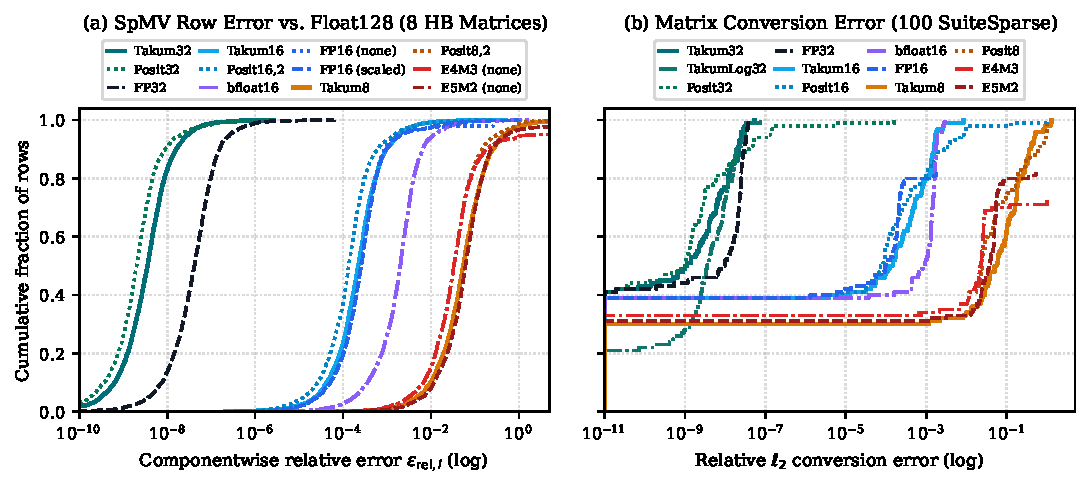
\includegraphics[width=0.72\textwidth]{figures/error-cdf.pdf}
\caption{Empirical CDFs: (a) componentwise SpMV row errors against \texttt{Float128} across 8 Harwell-Boeing matrices (94,276 row evaluations; unscaled \texttt{E4M3}, \texttt{E5M2}, and \texttt{FP16} plateau below 1.0 due to overflows), and (b) matrix conversion $\ell_2$ error across 100 SuiteSparse matrices (80-bit \texttt{long double} reference) comparing 15 formats including \texttt{Posit} ($es=2$) and logarithmic Takum.}
\label{fig:error_cdf}
\end{figure*}

\subsection{100 SuiteSparse Matrices and Logarithmic Takum}
\begin{table}[t]
\caption{Conversion viability across 100 SuiteSparse matrices ($\mathrm{nnz} \le 50\,000$ declared, 80-bit \texttt{long double} reference): Takum (Linear and Logarithmic), Posit ($es=2$), and IEEE/OCP formats.}
\label{tab:suitesparse100}
\centering
\scriptsize
\setlength{\tabcolsep}{3.0pt}
\renewcommand{\arraystretch}{0.95}
\begin{tabular}{@{}lcccc@{}}
\toprule
Format & Fin. & Median & P90 & Max \\
\midrule
OFP8 E4M3 & 73/100 & $7.17 \times 10^{-3}$ & $2.70 \times 10^{-2}$ & $1.00 \times 10^{0}$ \\
OFP8 E5M2 & 82/100 & $2.39 \times 10^{-2}$ & $5.63 \times 10^{-2}$ & $5.33 \times 10^{-1}$ \\
Posit8 & 100/100 & $2.45 \times 10^{-2}$ & $6.13 \times 10^{-1}$ & $1.07 \times 10^{0}$ \\
Takum8 (Lin.) & 100/100 & $5.35 \times 10^{-2}$ & $3.66 \times 10^{-1}$ & $1.30 \times 10^{0}$ \\
Takum8 (Log) & 100/100 & $5.42 \times 10^{-2}$ & $3.61 \times 10^{-1}$ & $3.26 \times 10^{0}$ \\
\midrule
IEEE FP16 & 82/100 & $7.58 \times 10^{-6}$ & $2.18 \times 10^{-4}$ & $1.80 \times 10^{-3}$ \\
bfloat16 & 100/100 & $8.87 \times 10^{-4}$ & $1.76 \times 10^{-3}$ & $2.96 \times 10^{-3}$ \\
Posit16 & 100/100 & $7.89 \times 10^{-5}$ & $2.79 \times 10^{-3}$ & $9.99 \times 10^{-1}$ \\
Takum16 (Lin.) & 100/100 & $1.34 \times 10^{-4}$ & $1.57 \times 10^{-3}$ & $8.49 \times 10^{-3}$ \\
Takum16 (Log) & 100/100 & $2.17 \times 10^{-4}$ & $1.31 \times 10^{-3}$ & $7.48 \times 10^{-3}$ \\
\midrule
IEEE FP32 & 100/100 & $9.64 \times 10^{-9}$ & $2.97 \times 10^{-8}$ & $4.08 \times 10^{-8}$ \\
Posit32 & 100/100 & $9.88 \times 10^{-10}$ & $3.14 \times 10^{-8}$ & $1.59 \times 10^{-4}$ \\
Takum32 (Lin.) & 100/100 & $1.06 \times 10^{-9}$ & $2.14 \times 10^{-8}$ & $5.42 \times 10^{-8}$ \\
Takum32 (Log) & 100/100 & $3.59 \times 10^{-9}$ & $1.87 \times 10^{-8}$ & $7.57 \times 10^{-8}$ \\
\bottomrule
\end{tabular}
\end{table}

Figure~\ref{fig:error_cdf}(b) and Table~\ref{tab:suitesparse100} extend representation analysis to 100 SuiteSparse matrices. While \texttt{Posit} attains lower median conversion error near unity (\texttt{Posit16}: $7.89\times 10^{-5}$ vs.\ \texttt{Takum16}: $1.34\times 10^{-4}$), its exponential precision collapse yields 99.9\% maximum error in \texttt{Posit16} (vs.\ 0.85\% in \texttt{Takum16}) and $1.59\times 10^{-4}$ in \texttt{Posit32} (vs.\ $5.42\times 10^{-8}$ in \texttt{Takum32}). Logarithmic Takum tracks linear Takum across all widths~\cite{hunhold2024takum}.

\subsection{Instruction Counts, CSR Writes, and Analytic Model}
\begin{table}[t]
\caption{Dynamic instructions, \texttt{Zvtakum} instructions, CSR writes, and active elements per nonzero, aggregated over all eight Harwell--Boeing matrices.}
\label{tab:contagens}
\centering
\scriptsize
\setlength{\tabcolsep}{3.0pt}
\renewcommand{\arraystretch}{0.95}
\begin{tabular}{@{}llcccc@{}}
\toprule
Fmt & VLEN & Insn/nnz & Zvt./nnz & CSR/nnz & Elem./nnz \\
\midrule
FP32 & 128 & 6.140 & 0.000 & 1.328 & 5.334 \\
FP32 & 256 & 4.587 & 0.000 & 1.069 & 5.334 \\
FP32 & 512 & 4.343 & 0.000 & 1.029 & 5.334 \\
\midrule
Takum32 & 128 & 5.977 & 0.497 & 1.328 & 4.501 \\
Takum32 & 256 & 4.553 & 0.368 & 1.069 & 4.501 \\
Takum32 & 512 & 4.329 & 0.347 & 1.029 & 4.501 \\
\midrule
Takum16 & 128 & 4.954 & 0.368 & 1.470 & 4.501 \\
Takum16 & 256 & 4.690 & 0.347 & 1.389 & 4.501 \\
Takum16 & 512 & 4.605 & 0.341 & 1.363 & 4.501 \\
\midrule
Takum8 & 128 & 4.510 & 0.347 & 1.389 & 4.501 \\
Takum8 & 256 & 4.431 & 0.341 & 1.363 & 4.501 \\
Takum8 & 512 & 4.392 & 0.337 & 1.350 & 4.501 \\
\bottomrule
\end{tabular}
\end{table}

\begin{table}[t]
\caption{Parameters of the analytic instruction-count model $N_f = r_f R + c_f S + K$, where $R$ is row count and $S$ is total nonempty-row strip count across all 96 simulator runs.}
\label{tab:modelo}
\centering
\scriptsize
\setlength{\tabcolsep}{3.0pt}
\renewcommand{\arraystretch}{0.95}
\begin{tabular}{@{}lcccrr@{}}
\toprule
Format & $r$ & $c$ & $K$ & Synthetic & Exact runs \\
\midrule
FP32 & 13 & 12 & 21 & 3/3 & 24/24 \\
Takum8 & 14 & 12 & 21 & 3/3 & 24/24 \\
Takum16 & 14 & 13 & 21 & 3/3 & 24/24 \\
Takum32 & 14 & 11 & 21 & 3/3 & 24/24 \\
\bottomrule
\end{tabular}
\end{table}

\begin{figure}[t]
\centering
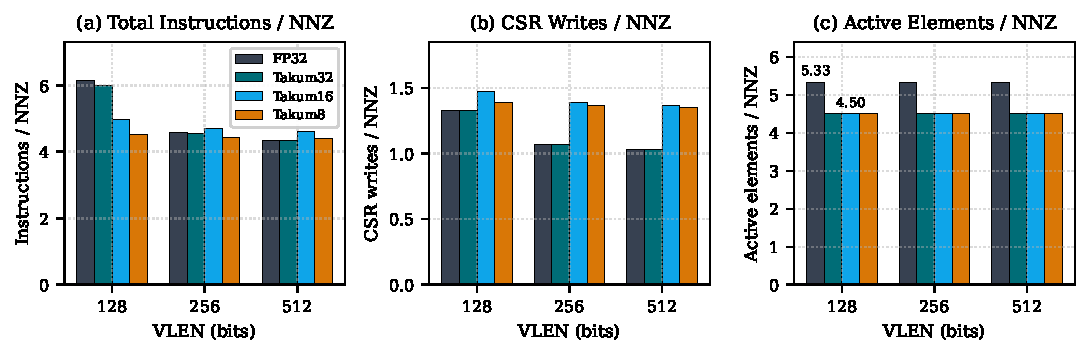
\includegraphics[width=0.75\columnwidth]{figures/insn-csr-comparison.pdf}
\caption{Dynamic instructions, CSR writes, and active vector elements per nonzero across $\mathrm{VLEN}\in\{128,256,512\}$ summed over all eight matrices.}
\label{fig:insn_csr}
\end{figure}

All \NumBitExatas\ simulator SpMV runs match our Python reference bitwise. Tables~\ref{tab:contagens} and~\ref{tab:modelo} and Fig.~\ref{fig:insn_csr} satisfy the exact identity $N_f = r_f R + c_f S + K$ with \ModResiduoMax\ residual across all \ModExec\ real runs ($R$ rows, $S$ nonempty strips, $K=\ModKFP$). Since \texttt{vtdot.vv} merges \texttt{vfmul.vv} and \texttt{vfredusum.vs} ($c_{\text{T32}}=11 < c_{\text{FP32}}=12$) while \texttt{vncvt.t.t} adds one per-row instruction ($r_{\text{T32}}=14$ vs.\ $r_{\text{FP32}}=13$), their kernel difference is $N_{\text{Takum32}} - N_{\text{FP32}} = R - S \le 0$. Thus \texttt{Takum32} uses fewer or equal instructions across all \InsnPares\ pairs (\InsnMenorTrinta\ fewer, \InsnIgualTrinta\ equal), issues identical CSR writes to \texttt{FP32} (\CsrNnzTrintaDuzentos/nnz at $\mathrm{VLEN}=256$), and lowers active elements per nonzero from \ElemNnzFP\ to \ElemNnzTakum\ ($-15.6\%$). For 8 and 16 bits, switching \texttt{vtype} between 32-bit CSR indices and narrow data adds one \texttt{vsetvli} per strip ($+27\%\text{--}33\%$ CSR writes at $\mathrm{VLEN}=256$), though wider vector packing at $\mathrm{VLEN}=128$ reduces total instructions by \RelInsnDezCento\ (\texttt{Takum16}) and \RelInsnOitoCento\ (\texttt{Takum8}).

\subsection{Limitations}
This evaluation uses a functional, unpipelined simulator without cycle timing, silicon area, or power synthesis. \texttt{FP8}, \texttt{FP16}, \texttt{bfloat16}, and \texttt{Posit} SpMV metrics reflect software numerical baselines rather than executed hardware kernels (such as \texttt{Zvfh}). The SpMV workload covers eight small-to-medium Harwell-Boeing matrices ($\le 1{,}033$ rows), so aggregate medians are sensitive to matrix scale distributions; in particular, \texttt{Posit8,2} outperforms \texttt{Takum8} on 7/8 matrices in this sample. Host-side \texttt{pow2-bound} scaling requires two global reduction passes excluded from vector counters, and the 100-matrix SuiteSparse conversion CSV uses 80-bit \texttt{long double} because bulk downloads from \texttt{sparse.tamu.edu} were unavailable (\texttt{HTTP 403}) during offline audit.

\section{Conclusion}
We presented and verified the \texttt{Zvtakum} RVV extension supporting \texttt{T8}, \texttt{T16}, and \texttt{T32} via five \texttt{custom-0} instructions, a unified 12-MSB decoder, a 128-bit integer ALU with code-space RNE, and no \texttt{fcsr} hazards. On Harwell-Boeing SpMV, \texttt{Takum32} lowers median relative error by $\RazaoKernelTrinta\times$ over \texttt{FP32} while never exceeding \texttt{FP32} instruction counts, \texttt{Takum8}/\texttt{Takum16} prevent non-finite overflows without pre-scaling, \texttt{Takum16} outperforms \texttt{bfloat16}, and \texttt{Takum} avoids the extreme-scale precision collapse observed in posits.

\bibliographystyle{IEEEtran}
\bibliography{refs}
\end{document}
